\begin{figure}[htbp]
\centering
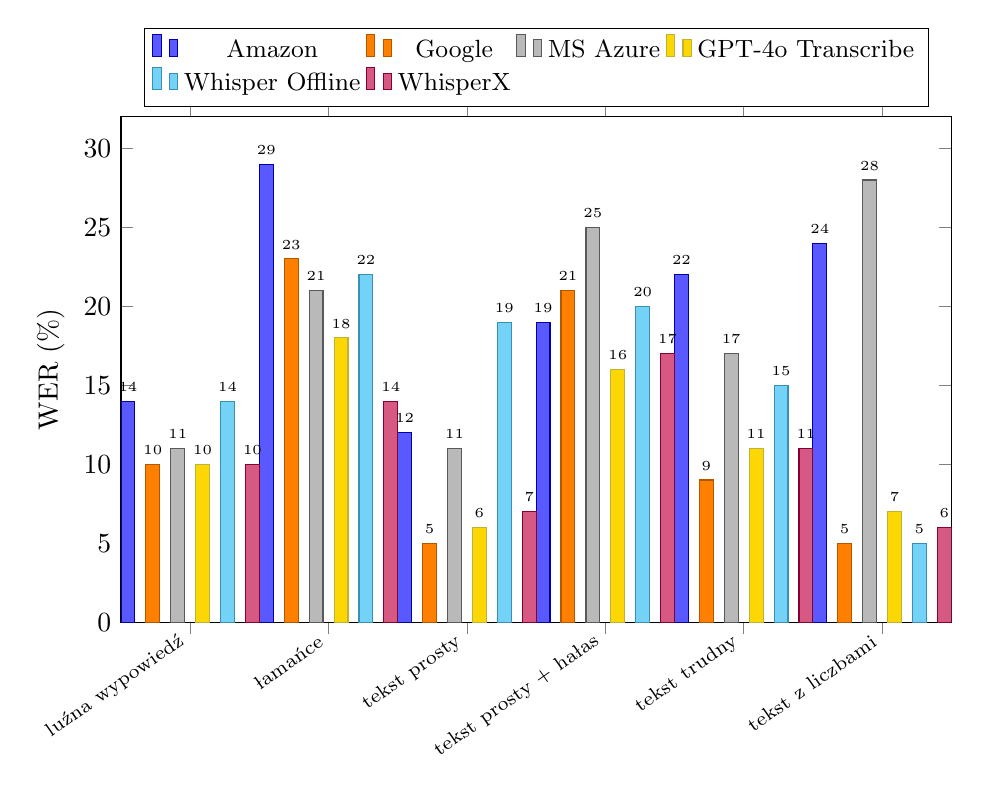
\begin{tikzpicture}
\begin{axis}[
    ybar=4pt,
    bar width=5pt,
    symbolic x coords={
        luźna wypowiedź,
        łamańce,
        tekst prosty,
        tekst prosty + hałas,
        tekst trudny,
        tekst z liczbami
    },
    xtick=data,
    nodes near coords,
    nodes near coords align={vertical},
    nodes near coords style={
        /pgf/number format/fixed,
        /pgf/number format/precision=0,
        font=\tiny,
    },
    ylabel={WER (\%)},
    ymin=0, ymax=32,
    ytick={0,5,10,15,20,25,30},
    yticklabel={\pgfmathprintnumber[fixed,precision=0]{\tick}},
    enlarge x limits=0.10,
    title={WER (\%) - wpływ typu materiału słownego},
    legend style={
        at={(0.5,1.02)},
        anchor=south,
        legend columns=4,
        font=\small,
    },
    x tick label style={
        rotate=35,
        anchor=east,
        align=center,
        font=\scriptsize,
    },
    width=1.0\textwidth,
    height=8cm,
]
\addplot[fill=blue!65, draw=blue!65!black] coordinates {
    (luźna wypowiedź,14)
    (łamańce,29)
    (tekst prosty,12)
    (tekst prosty + hałas,19)
    (tekst trudny,22)
    (tekst z liczbami,24)
};
\addplot[fill=orange, draw=orange!70!black] coordinates {
    (luźna wypowiedź,10)
    (łamańce,23)
    (tekst prosty,5)
    (tekst prosty + hałas,21)
    (tekst trudny,9)
    (tekst z liczbami,5)
};
\addplot[fill=gray!55, draw=gray!70!black] coordinates {
    (luźna wypowiedź,11)
    (łamańce,21)
    (tekst prosty,11)
    (tekst prosty + hałas,25)
    (tekst trudny,17)
    (tekst z liczbami,28)
};
\addplot[fill=yellow!75!orange, draw=yellow!70!black] coordinates {
    (luźna wypowiedź,10)
    (łamańce,18)
    (tekst prosty,6)
    (tekst prosty + hałas,16)
    (tekst trudny,11)
    (tekst z liczbami,7)
};
\addplot[fill=cyan!55, draw=cyan!70!black] coordinates {
    (luźna wypowiedź,14)
    (łamańce,22)
    (tekst prosty,19)
    (tekst prosty + hałas,20)
    (tekst trudny,15)
    (tekst z liczbami,5)
};
\addplot[fill=purple!65, draw=purple!70!black] coordinates {
    (luźna wypowiedź,10)
    (łamańce,14)
    (tekst prosty,7)
    (tekst prosty + hałas,17)
    (tekst trudny,11)
    (tekst z liczbami,6)
};
\legend{Amazon,Google,MS Azure,GPT-4o Transcribe,Whisper Offline,WhisperX}
\end{axis}
\end{tikzpicture}
\caption{Porównanie błędu WER dla badanych modeli ASR w zależności od typu materiału słownego.}
\label{fig:wer_text_type_comparison}
\end{figure}
